% Created by tikzDevice version 0.12.6 on 2024-10-05 16:18:00
% !TEX encoding = UTF-8 Unicode
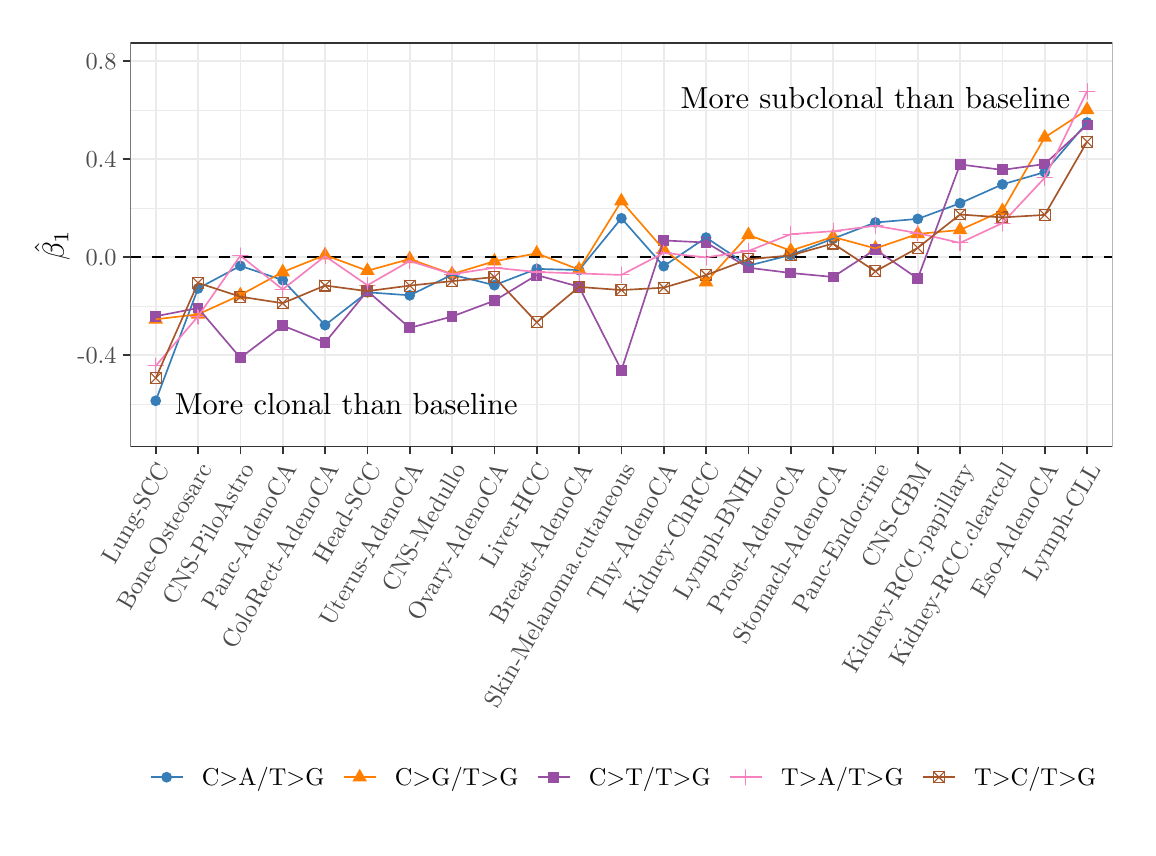
\begin{tikzpicture}[x=1pt,y=1pt]
\definecolor{fillColor}{RGB}{255,255,255}
\path[use as bounding box,fill=fillColor,fill opacity=0.00] (0,0) rectangle (397.48,289.08);
\begin{scope}
\path[clip] (  0.00,  0.00) rectangle (397.48,289.08);
\definecolor{drawColor}{RGB}{255,255,255}
\definecolor{fillColor}{RGB}{255,255,255}

\path[draw=drawColor,line width= 0.6pt,line join=round,line cap=round,fill=fillColor] (  0.00, -0.00) rectangle (397.48,289.08);
\end{scope}
\begin{scope}
\path[clip] ( 37.09,137.61) rectangle (391.98,283.58);
\definecolor{fillColor}{RGB}{255,255,255}

\path[fill=fillColor] ( 37.09,137.61) rectangle (391.98,283.58);
\definecolor{drawColor}{gray}{0.92}

\path[draw=drawColor,line width= 0.3pt,line join=round] ( 37.09,153.09) --
	(391.98,153.09);

\path[draw=drawColor,line width= 0.3pt,line join=round] ( 37.09,188.48) --
	(391.98,188.48);

\path[draw=drawColor,line width= 0.3pt,line join=round] ( 37.09,223.86) --
	(391.98,223.86);

\path[draw=drawColor,line width= 0.3pt,line join=round] ( 37.09,259.25) --
	(391.98,259.25);

\path[draw=drawColor,line width= 0.6pt,line join=round] ( 37.09,170.78) --
	(391.98,170.78);

\path[draw=drawColor,line width= 0.6pt,line join=round] ( 37.09,206.17) --
	(391.98,206.17);

\path[draw=drawColor,line width= 0.6pt,line join=round] ( 37.09,241.56) --
	(391.98,241.56);

\path[draw=drawColor,line width= 0.6pt,line join=round] ( 37.09,276.94) --
	(391.98,276.94);

\path[draw=drawColor,line width= 0.6pt,line join=round] ( 46.27,137.61) --
	( 46.27,283.58);

\path[draw=drawColor,line width= 0.6pt,line join=round] ( 61.56,137.61) --
	( 61.56,283.58);

\path[draw=drawColor,line width= 0.6pt,line join=round] ( 76.86,137.61) --
	( 76.86,283.58);

\path[draw=drawColor,line width= 0.6pt,line join=round] ( 92.16,137.61) --
	( 92.16,283.58);

\path[draw=drawColor,line width= 0.6pt,line join=round] (107.46,137.61) --
	(107.46,283.58);

\path[draw=drawColor,line width= 0.6pt,line join=round] (122.75,137.61) --
	(122.75,283.58);

\path[draw=drawColor,line width= 0.6pt,line join=round] (138.05,137.61) --
	(138.05,283.58);

\path[draw=drawColor,line width= 0.6pt,line join=round] (153.35,137.61) --
	(153.35,283.58);

\path[draw=drawColor,line width= 0.6pt,line join=round] (168.65,137.61) --
	(168.65,283.58);

\path[draw=drawColor,line width= 0.6pt,line join=round] (183.94,137.61) --
	(183.94,283.58);

\path[draw=drawColor,line width= 0.6pt,line join=round] (199.24,137.61) --
	(199.24,283.58);

\path[draw=drawColor,line width= 0.6pt,line join=round] (214.54,137.61) --
	(214.54,283.58);

\path[draw=drawColor,line width= 0.6pt,line join=round] (229.83,137.61) --
	(229.83,283.58);

\path[draw=drawColor,line width= 0.6pt,line join=round] (245.13,137.61) --
	(245.13,283.58);

\path[draw=drawColor,line width= 0.6pt,line join=round] (260.43,137.61) --
	(260.43,283.58);

\path[draw=drawColor,line width= 0.6pt,line join=round] (275.73,137.61) --
	(275.73,283.58);

\path[draw=drawColor,line width= 0.6pt,line join=round] (291.02,137.61) --
	(291.02,283.58);

\path[draw=drawColor,line width= 0.6pt,line join=round] (306.32,137.61) --
	(306.32,283.58);

\path[draw=drawColor,line width= 0.6pt,line join=round] (321.62,137.61) --
	(321.62,283.58);

\path[draw=drawColor,line width= 0.6pt,line join=round] (336.91,137.61) --
	(336.91,283.58);

\path[draw=drawColor,line width= 0.6pt,line join=round] (352.21,137.61) --
	(352.21,283.58);

\path[draw=drawColor,line width= 0.6pt,line join=round] (367.51,137.61) --
	(367.51,283.58);

\path[draw=drawColor,line width= 0.6pt,line join=round] (382.81,137.61) --
	(382.81,283.58);
\definecolor{fillColor}{RGB}{55,126,184}

\path[fill=fillColor] ( 61.56,194.84) circle (  1.96);
\definecolor{fillColor}{RGB}{255,127,0}

\path[fill=fillColor] ( 61.56,188.54) --
	( 64.21,183.96) --
	( 58.92,183.96) --
	cycle;
\definecolor{fillColor}{RGB}{152,78,163}

\path[fill=fillColor] ( 59.60,185.81) --
	( 63.53,185.81) --
	( 63.53,189.73) --
	( 59.60,189.73) --
	cycle;
\definecolor{drawColor}{RGB}{247,129,191}

\path[draw=drawColor,line width= 0.4pt,line join=round,line cap=round] ( 58.79,184.77) -- ( 64.34,184.77);

\path[draw=drawColor,line width= 0.4pt,line join=round,line cap=round] ( 61.56,182.00) -- ( 61.56,187.55);
\definecolor{drawColor}{RGB}{166,86,40}

\path[draw=drawColor,line width= 0.4pt,line join=round,line cap=round] ( 59.60,194.89) rectangle ( 63.53,198.81);

\path[draw=drawColor,line width= 0.4pt,line join=round,line cap=round] ( 59.60,194.89) -- ( 63.53,198.81);

\path[draw=drawColor,line width= 0.4pt,line join=round,line cap=round] ( 59.60,198.81) -- ( 63.53,194.89);
\definecolor{fillColor}{RGB}{55,126,184}

\path[fill=fillColor] (199.24,201.50) circle (  1.96);
\definecolor{fillColor}{RGB}{255,127,0}

\path[fill=fillColor] (199.24,204.74) --
	(201.88,200.16) --
	(196.60,200.16) --
	cycle;
\definecolor{fillColor}{RGB}{152,78,163}

\path[fill=fillColor] (197.28,193.51) --
	(201.20,193.51) --
	(201.20,197.43) --
	(197.28,197.43) --
	cycle;
\definecolor{drawColor}{RGB}{247,129,191}

\path[draw=drawColor,line width= 0.4pt,line join=round,line cap=round] (196.46,200.26) -- (202.01,200.26);

\path[draw=drawColor,line width= 0.4pt,line join=round,line cap=round] (199.24,197.49) -- (199.24,203.04);
\definecolor{drawColor}{RGB}{166,86,40}

\path[draw=drawColor,line width= 0.4pt,line join=round,line cap=round] (197.28,193.43) rectangle (201.20,197.35);

\path[draw=drawColor,line width= 0.4pt,line join=round,line cap=round] (197.28,193.43) -- (201.20,197.35);

\path[draw=drawColor,line width= 0.4pt,line join=round,line cap=round] (197.28,197.35) -- (201.20,193.43);
\definecolor{fillColor}{RGB}{55,126,184}

\path[fill=fillColor] (321.62,219.97) circle (  1.96);
\definecolor{fillColor}{RGB}{255,127,0}

\path[fill=fillColor] (321.62,217.59) --
	(324.26,213.02) --
	(318.98,213.02) --
	cycle;
\definecolor{fillColor}{RGB}{152,78,163}

\path[fill=fillColor] (319.66,196.46) --
	(323.58,196.46) --
	(323.58,200.38) --
	(319.66,200.38) --
	cycle;
\definecolor{drawColor}{RGB}{247,129,191}

\path[draw=drawColor,line width= 0.4pt,line join=round,line cap=round] (318.84,214.85) -- (324.39,214.85);

\path[draw=drawColor,line width= 0.4pt,line join=round,line cap=round] (321.62,212.07) -- (321.62,217.62);
\definecolor{drawColor}{RGB}{166,86,40}

\path[draw=drawColor,line width= 0.4pt,line join=round,line cap=round] (319.66,207.55) rectangle (323.58,211.47);

\path[draw=drawColor,line width= 0.4pt,line join=round,line cap=round] (319.66,207.55) -- (323.58,211.47);

\path[draw=drawColor,line width= 0.4pt,line join=round,line cap=round] (319.66,211.47) -- (323.58,207.55);
\definecolor{fillColor}{RGB}{55,126,184}

\path[fill=fillColor] (153.35,199.81) circle (  1.96);
\definecolor{fillColor}{RGB}{255,127,0}

\path[fill=fillColor] (153.35,203.08) --
	(155.99,198.51) --
	(150.71,198.51) --
	cycle;
\definecolor{fillColor}{RGB}{152,78,163}

\path[fill=fillColor] (151.39,182.75) --
	(155.31,182.75) --
	(155.31,186.67) --
	(151.39,186.67) --
	cycle;
\definecolor{drawColor}{RGB}{247,129,191}

\path[draw=drawColor,line width= 0.4pt,line join=round,line cap=round] (150.57,199.99) -- (156.12,199.99);

\path[draw=drawColor,line width= 0.4pt,line join=round,line cap=round] (153.35,197.22) -- (153.35,202.77);
\definecolor{drawColor}{RGB}{166,86,40}

\path[draw=drawColor,line width= 0.4pt,line join=round,line cap=round] (151.39,195.53) rectangle (155.31,199.45);

\path[draw=drawColor,line width= 0.4pt,line join=round,line cap=round] (151.39,195.53) -- (155.31,199.45);

\path[draw=drawColor,line width= 0.4pt,line join=round,line cap=round] (151.39,199.45) -- (155.31,195.53);
\definecolor{fillColor}{RGB}{55,126,184}

\path[fill=fillColor] ( 76.86,203.02) circle (  1.96);
\definecolor{fillColor}{RGB}{255,127,0}

\path[fill=fillColor] ( 76.86,195.50) --
	( 79.50,190.92) --
	( 74.22,190.92) --
	cycle;
\definecolor{fillColor}{RGB}{152,78,163}

\path[fill=fillColor] ( 74.90,167.82) --
	( 78.82,167.82) --
	( 78.82,171.74) --
	( 74.90,171.74) --
	cycle;
\definecolor{drawColor}{RGB}{247,129,191}

\path[draw=drawColor,line width= 0.4pt,line join=round,line cap=round] ( 74.09,206.69) -- ( 79.64,206.69);

\path[draw=drawColor,line width= 0.4pt,line join=round,line cap=round] ( 76.86,203.92) -- ( 76.86,209.47);
\definecolor{drawColor}{RGB}{166,86,40}

\path[draw=drawColor,line width= 0.4pt,line join=round,line cap=round] ( 74.90,189.90) rectangle ( 78.82,193.83);

\path[draw=drawColor,line width= 0.4pt,line join=round,line cap=round] ( 74.90,189.90) -- ( 78.82,193.83);

\path[draw=drawColor,line width= 0.4pt,line join=round,line cap=round] ( 74.90,193.83) -- ( 78.82,189.90);
\definecolor{fillColor}{RGB}{55,126,184}

\path[fill=fillColor] (107.46,181.59) circle (  1.96);
\definecolor{fillColor}{RGB}{255,127,0}

\path[fill=fillColor] (107.46,209.95) --
	(110.10,205.38) --
	(104.81,205.38) --
	cycle;
\definecolor{fillColor}{RGB}{152,78,163}

\path[fill=fillColor] (105.49,173.37) --
	(109.42,173.37) --
	(109.42,177.29) --
	(105.49,177.29) --
	cycle;
\definecolor{drawColor}{RGB}{247,129,191}

\path[draw=drawColor,line width= 0.4pt,line join=round,line cap=round] (104.68,206.53) -- (110.23,206.53);

\path[draw=drawColor,line width= 0.4pt,line join=round,line cap=round] (107.46,203.76) -- (107.46,209.31);
\definecolor{drawColor}{RGB}{166,86,40}

\path[draw=drawColor,line width= 0.4pt,line join=round,line cap=round] (105.49,193.94) rectangle (109.42,197.87);

\path[draw=drawColor,line width= 0.4pt,line join=round,line cap=round] (105.49,193.94) -- (109.42,197.87);

\path[draw=drawColor,line width= 0.4pt,line join=round,line cap=round] (105.49,197.87) -- (109.42,193.94);
\definecolor{fillColor}{RGB}{55,126,184}

\path[fill=fillColor] (367.51,236.87) circle (  1.96);
\definecolor{fillColor}{RGB}{255,127,0}

\path[fill=fillColor] (367.51,252.46) --
	(370.15,247.88) --
	(364.87,247.88) --
	cycle;
\definecolor{fillColor}{RGB}{152,78,163}

\path[fill=fillColor] (365.55,237.84) --
	(369.47,237.84) --
	(369.47,241.77) --
	(365.55,241.77) --
	cycle;
\definecolor{drawColor}{RGB}{247,129,191}

\path[draw=drawColor,line width= 0.4pt,line join=round,line cap=round] (364.73,234.85) -- (370.28,234.85);

\path[draw=drawColor,line width= 0.4pt,line join=round,line cap=round] (367.51,232.07) -- (367.51,237.62);
\definecolor{drawColor}{RGB}{166,86,40}

\path[draw=drawColor,line width= 0.4pt,line join=round,line cap=round] (365.55,219.46) rectangle (369.47,223.38);

\path[draw=drawColor,line width= 0.4pt,line join=round,line cap=round] (365.55,219.46) -- (369.47,223.38);

\path[draw=drawColor,line width= 0.4pt,line join=round,line cap=round] (365.55,223.38) -- (369.47,219.46);
\definecolor{fillColor}{RGB}{55,126,184}

\path[fill=fillColor] (122.75,193.46) circle (  1.96);
\definecolor{fillColor}{RGB}{255,127,0}

\path[fill=fillColor] (122.75,204.30) --
	(125.40,199.72) --
	(120.11,199.72) --
	cycle;
\definecolor{fillColor}{RGB}{152,78,163}

\path[fill=fillColor] (120.79,191.96) --
	(124.72,191.96) --
	(124.72,195.89) --
	(120.79,195.89) --
	cycle;
\definecolor{drawColor}{RGB}{247,129,191}

\path[draw=drawColor,line width= 0.4pt,line join=round,line cap=round] (119.98,196.00) -- (125.53,196.00);

\path[draw=drawColor,line width= 0.4pt,line join=round,line cap=round] (122.75,193.22) -- (122.75,198.77);
\definecolor{drawColor}{RGB}{166,86,40}

\path[draw=drawColor,line width= 0.4pt,line join=round,line cap=round] (120.79,191.91) rectangle (124.72,195.84);

\path[draw=drawColor,line width= 0.4pt,line join=round,line cap=round] (120.79,191.91) -- (124.72,195.84);

\path[draw=drawColor,line width= 0.4pt,line join=round,line cap=round] (120.79,195.84) -- (124.72,191.91);
\definecolor{fillColor}{RGB}{55,126,184}

\path[fill=fillColor] (245.13,213.22) circle (  1.96);
\definecolor{fillColor}{RGB}{255,127,0}

\path[fill=fillColor] (245.13,200.21) --
	(247.77,195.63) --
	(242.49,195.63) --
	cycle;
\definecolor{fillColor}{RGB}{152,78,163}

\path[fill=fillColor] (243.17,209.48) --
	(247.09,209.48) --
	(247.09,213.41) --
	(243.17,213.41) --
	cycle;
\definecolor{drawColor}{RGB}{247,129,191}

\path[draw=drawColor,line width= 0.4pt,line join=round,line cap=round] (242.36,206.08) -- (247.91,206.08);

\path[draw=drawColor,line width= 0.4pt,line join=round,line cap=round] (245.13,203.30) -- (245.13,208.85);
\definecolor{drawColor}{RGB}{166,86,40}

\path[draw=drawColor,line width= 0.4pt,line join=round,line cap=round] (243.17,197.71) rectangle (247.09,201.64);

\path[draw=drawColor,line width= 0.4pt,line join=round,line cap=round] (243.17,197.71) -- (247.09,201.64);

\path[draw=drawColor,line width= 0.4pt,line join=round,line cap=round] (243.17,201.64) -- (247.09,197.71);
\definecolor{fillColor}{RGB}{55,126,184}

\path[fill=fillColor] (352.21,232.45) circle (  1.96);
\definecolor{fillColor}{RGB}{255,127,0}

\path[fill=fillColor] (352.21,225.93) --
	(354.85,221.36) --
	(349.57,221.36) --
	cycle;
\definecolor{fillColor}{RGB}{152,78,163}

\path[fill=fillColor] (350.25,235.72) --
	(354.17,235.72) --
	(354.17,239.65) --
	(350.25,239.65) --
	cycle;
\definecolor{drawColor}{RGB}{247,129,191}

\path[draw=drawColor,line width= 0.4pt,line join=round,line cap=round] (349.44,218.46) -- (354.99,218.46);

\path[draw=drawColor,line width= 0.4pt,line join=round,line cap=round] (352.21,215.69) -- (352.21,221.24);
\definecolor{drawColor}{RGB}{166,86,40}

\path[draw=drawColor,line width= 0.4pt,line join=round,line cap=round] (350.25,218.55) rectangle (354.17,222.48);

\path[draw=drawColor,line width= 0.4pt,line join=round,line cap=round] (350.25,218.55) -- (354.17,222.48);

\path[draw=drawColor,line width= 0.4pt,line join=round,line cap=round] (350.25,222.48) -- (354.17,218.55);
\definecolor{fillColor}{RGB}{55,126,184}

\path[fill=fillColor] (336.91,225.63) circle (  1.96);
\definecolor{fillColor}{RGB}{255,127,0}

\path[fill=fillColor] (336.91,219.02) --
	(339.56,214.44) --
	(334.27,214.44) --
	cycle;
\definecolor{fillColor}{RGB}{152,78,163}

\path[fill=fillColor] (334.95,237.70) --
	(338.88,237.70) --
	(338.88,241.62) --
	(334.95,241.62) --
	cycle;
\definecolor{drawColor}{RGB}{247,129,191}

\path[draw=drawColor,line width= 0.4pt,line join=round,line cap=round] (334.14,211.31) -- (339.69,211.31);

\path[draw=drawColor,line width= 0.4pt,line join=round,line cap=round] (336.91,208.53) -- (336.91,214.08);
\definecolor{drawColor}{RGB}{166,86,40}

\path[draw=drawColor,line width= 0.4pt,line join=round,line cap=round] (334.95,219.61) rectangle (338.88,223.53);

\path[draw=drawColor,line width= 0.4pt,line join=round,line cap=round] (334.95,219.61) -- (338.88,223.53);

\path[draw=drawColor,line width= 0.4pt,line join=round,line cap=round] (334.95,223.53) -- (338.88,219.61);
\definecolor{fillColor}{RGB}{55,126,184}

\path[fill=fillColor] (183.94,201.92) circle (  1.96);
\definecolor{fillColor}{RGB}{255,127,0}

\path[fill=fillColor] (183.94,210.57) --
	(186.58,205.99) --
	(181.30,205.99) --
	cycle;
\definecolor{fillColor}{RGB}{152,78,163}

\path[fill=fillColor] (181.98,197.70) --
	(185.90,197.70) --
	(185.90,201.63) --
	(181.98,201.63) --
	cycle;
\definecolor{drawColor}{RGB}{247,129,191}

\path[draw=drawColor,line width= 0.4pt,line join=round,line cap=round] (181.17,200.78) -- (186.72,200.78);

\path[draw=drawColor,line width= 0.4pt,line join=round,line cap=round] (183.94,198.00) -- (183.94,203.55);
\definecolor{drawColor}{RGB}{166,86,40}

\path[draw=drawColor,line width= 0.4pt,line join=round,line cap=round] (181.98,180.64) rectangle (185.90,184.57);

\path[draw=drawColor,line width= 0.4pt,line join=round,line cap=round] (181.98,180.64) -- (185.90,184.57);

\path[draw=drawColor,line width= 0.4pt,line join=round,line cap=round] (181.98,184.57) -- (185.90,180.64);
\definecolor{fillColor}{RGB}{55,126,184}

\path[fill=fillColor] ( 46.27,154.25) circle (  1.96);
\definecolor{fillColor}{RGB}{255,127,0}

\path[fill=fillColor] ( 46.27,186.76) --
	( 48.91,182.18) --
	( 43.62,182.18) --
	cycle;
\definecolor{fillColor}{RGB}{152,78,163}

\path[fill=fillColor] ( 44.30,182.83) --
	( 48.23,182.83) --
	( 48.23,186.75) --
	( 44.30,186.75) --
	cycle;
\definecolor{drawColor}{RGB}{247,129,191}

\path[draw=drawColor,line width= 0.4pt,line join=round,line cap=round] ( 43.49,166.85) -- ( 49.04,166.85);

\path[draw=drawColor,line width= 0.4pt,line join=round,line cap=round] ( 46.27,164.08) -- ( 46.27,169.63);
\definecolor{drawColor}{RGB}{166,86,40}

\path[draw=drawColor,line width= 0.4pt,line join=round,line cap=round] ( 44.30,160.48) rectangle ( 48.23,164.41);

\path[draw=drawColor,line width= 0.4pt,line join=round,line cap=round] ( 44.30,160.48) -- ( 48.23,164.41);

\path[draw=drawColor,line width= 0.4pt,line join=round,line cap=round] ( 44.30,164.41) -- ( 48.23,160.48);
\definecolor{fillColor}{RGB}{55,126,184}

\path[fill=fillColor] (260.43,203.07) circle (  1.96);
\definecolor{fillColor}{RGB}{255,127,0}

\path[fill=fillColor] (260.43,217.22) --
	(263.07,212.64) --
	(257.79,212.64) --
	cycle;
\definecolor{fillColor}{RGB}{152,78,163}

\path[fill=fillColor] (258.47,200.38) --
	(262.39,200.38) --
	(262.39,204.30) --
	(258.47,204.30) --
	cycle;
\definecolor{drawColor}{RGB}{247,129,191}

\path[draw=drawColor,line width= 0.4pt,line join=round,line cap=round] (257.65,208.39) -- (263.20,208.39);

\path[draw=drawColor,line width= 0.4pt,line join=round,line cap=round] (260.43,205.61) -- (260.43,211.16);
\definecolor{drawColor}{RGB}{166,86,40}

\path[draw=drawColor,line width= 0.4pt,line join=round,line cap=round] (258.47,203.42) rectangle (262.39,207.35);

\path[draw=drawColor,line width= 0.4pt,line join=round,line cap=round] (258.47,203.42) -- (262.39,207.35);

\path[draw=drawColor,line width= 0.4pt,line join=round,line cap=round] (258.47,207.35) -- (262.39,203.42);
\definecolor{fillColor}{RGB}{55,126,184}

\path[fill=fillColor] (382.81,254.79) circle (  1.96);
\definecolor{fillColor}{RGB}{255,127,0}

\path[fill=fillColor] (382.81,262.45) --
	(385.45,257.88) --
	(380.16,257.88) --
	cycle;
\definecolor{fillColor}{RGB}{152,78,163}

\path[fill=fillColor] (380.84,251.95) --
	(384.77,251.95) --
	(384.77,255.88) --
	(380.84,255.88) --
	cycle;
\definecolor{drawColor}{RGB}{247,129,191}

\path[draw=drawColor,line width= 0.4pt,line join=round,line cap=round] (380.03,266.07) -- (385.58,266.07);

\path[draw=drawColor,line width= 0.4pt,line join=round,line cap=round] (382.81,263.29) -- (382.81,268.84);
\definecolor{drawColor}{RGB}{166,86,40}

\path[draw=drawColor,line width= 0.4pt,line join=round,line cap=round] (380.84,245.89) rectangle (384.77,249.82);

\path[draw=drawColor,line width= 0.4pt,line join=round,line cap=round] (380.84,245.89) -- (384.77,249.82);

\path[draw=drawColor,line width= 0.4pt,line join=round,line cap=round] (380.84,249.82) -- (384.77,245.89);
\definecolor{fillColor}{RGB}{55,126,184}

\path[fill=fillColor] (168.65,196.02) circle (  1.96);
\definecolor{fillColor}{RGB}{255,127,0}

\path[fill=fillColor] (168.65,207.72) --
	(171.29,203.14) --
	(166.00,203.14) --
	cycle;
\definecolor{fillColor}{RGB}{152,78,163}

\path[fill=fillColor] (166.68,188.45) --
	(170.61,188.45) --
	(170.61,192.38) --
	(166.68,192.38) --
	cycle;
\definecolor{drawColor}{RGB}{247,129,191}

\path[draw=drawColor,line width= 0.4pt,line join=round,line cap=round] (165.87,202.33) -- (171.42,202.33);

\path[draw=drawColor,line width= 0.4pt,line join=round,line cap=round] (168.65,199.56) -- (168.65,205.11);
\definecolor{drawColor}{RGB}{166,86,40}

\path[draw=drawColor,line width= 0.4pt,line join=round,line cap=round] (166.68,196.97) rectangle (170.61,200.89);

\path[draw=drawColor,line width= 0.4pt,line join=round,line cap=round] (166.68,196.97) -- (170.61,200.89);

\path[draw=drawColor,line width= 0.4pt,line join=round,line cap=round] (166.68,200.89) -- (170.61,196.97);
\definecolor{fillColor}{RGB}{55,126,184}

\path[fill=fillColor] ( 92.16,197.85) circle (  1.96);
\definecolor{fillColor}{RGB}{255,127,0}

\path[fill=fillColor] ( 92.16,203.82) --
	( 94.80,199.25) --
	( 89.52,199.25) --
	cycle;
\definecolor{fillColor}{RGB}{152,78,163}

\path[fill=fillColor] ( 90.20,179.46) --
	( 94.12,179.46) --
	( 94.12,183.39) --
	( 90.20,183.39) --
	cycle;
\definecolor{drawColor}{RGB}{247,129,191}

\path[draw=drawColor,line width= 0.4pt,line join=round,line cap=round] ( 89.38,194.50) -- ( 94.93,194.50);

\path[draw=drawColor,line width= 0.4pt,line join=round,line cap=round] ( 92.16,191.72) -- ( 92.16,197.27);
\definecolor{drawColor}{RGB}{166,86,40}

\path[draw=drawColor,line width= 0.4pt,line join=round,line cap=round] ( 90.20,187.54) rectangle ( 94.12,191.47);

\path[draw=drawColor,line width= 0.4pt,line join=round,line cap=round] ( 90.20,187.54) -- ( 94.12,191.47);

\path[draw=drawColor,line width= 0.4pt,line join=round,line cap=round] ( 90.20,191.47) -- ( 94.12,187.54);
\definecolor{fillColor}{RGB}{55,126,184}

\path[fill=fillColor] (306.32,218.68) circle (  1.96);
\definecolor{fillColor}{RGB}{255,127,0}

\path[fill=fillColor] (306.32,212.36) --
	(308.96,207.78) --
	(303.68,207.78) --
	cycle;
\definecolor{fillColor}{RGB}{152,78,163}

\path[fill=fillColor] (304.36,206.99) --
	(308.28,206.99) --
	(308.28,210.92) --
	(304.36,210.92) --
	cycle;
\definecolor{drawColor}{RGB}{247,129,191}

\path[draw=drawColor,line width= 0.4pt,line join=round,line cap=round] (303.55,217.49) -- (309.10,217.49);

\path[draw=drawColor,line width= 0.4pt,line join=round,line cap=round] (306.32,214.72) -- (306.32,220.27);
\definecolor{drawColor}{RGB}{166,86,40}

\path[draw=drawColor,line width= 0.4pt,line join=round,line cap=round] (304.36,199.07) rectangle (308.28,202.99);

\path[draw=drawColor,line width= 0.4pt,line join=round,line cap=round] (304.36,199.07) -- (308.28,202.99);

\path[draw=drawColor,line width= 0.4pt,line join=round,line cap=round] (304.36,202.99) -- (308.28,199.07);
\definecolor{fillColor}{RGB}{55,126,184}

\path[fill=fillColor] (275.73,206.94) circle (  1.96);
\definecolor{fillColor}{RGB}{255,127,0}

\path[fill=fillColor] (275.73,211.56) --
	(278.37,206.98) --
	(273.08,206.98) --
	cycle;
\definecolor{fillColor}{RGB}{152,78,163}

\path[fill=fillColor] (273.76,198.47) --
	(277.69,198.47) --
	(277.69,202.39) --
	(273.76,202.39) --
	cycle;
\definecolor{drawColor}{RGB}{247,129,191}

\path[draw=drawColor,line width= 0.4pt,line join=round,line cap=round] (272.95,214.45) -- (278.50,214.45);

\path[draw=drawColor,line width= 0.4pt,line join=round,line cap=round] (275.73,211.68) -- (275.73,217.23);
\definecolor{drawColor}{RGB}{166,86,40}

\path[draw=drawColor,line width= 0.4pt,line join=round,line cap=round] (273.76,204.83) rectangle (277.69,208.76);

\path[draw=drawColor,line width= 0.4pt,line join=round,line cap=round] (273.76,204.83) -- (277.69,208.76);

\path[draw=drawColor,line width= 0.4pt,line join=round,line cap=round] (273.76,208.76) -- (277.69,204.83);
\definecolor{fillColor}{RGB}{55,126,184}

\path[fill=fillColor] (214.54,220.19) circle (  1.96);
\definecolor{fillColor}{RGB}{255,127,0}

\path[fill=fillColor] (214.54,229.45) --
	(217.18,224.88) --
	(211.89,224.88) --
	cycle;
\definecolor{fillColor}{RGB}{152,78,163}

\path[fill=fillColor] (212.57,163.34) --
	(216.50,163.34) --
	(216.50,167.27) --
	(212.57,167.27) --
	cycle;
\definecolor{drawColor}{RGB}{247,129,191}

\path[draw=drawColor,line width= 0.4pt,line join=round,line cap=round] (211.76,199.73) -- (217.31,199.73);

\path[draw=drawColor,line width= 0.4pt,line join=round,line cap=round] (214.54,196.96) -- (214.54,202.51);
\definecolor{drawColor}{RGB}{166,86,40}

\path[draw=drawColor,line width= 0.4pt,line join=round,line cap=round] (212.57,192.30) rectangle (216.50,196.22);

\path[draw=drawColor,line width= 0.4pt,line join=round,line cap=round] (212.57,192.30) -- (216.50,196.22);

\path[draw=drawColor,line width= 0.4pt,line join=round,line cap=round] (212.57,196.22) -- (216.50,192.30);
\definecolor{fillColor}{RGB}{55,126,184}

\path[fill=fillColor] (291.02,212.84) circle (  1.96);
\definecolor{fillColor}{RGB}{255,127,0}

\path[fill=fillColor] (291.02,216.52) --
	(293.67,211.95) --
	(288.38,211.95) --
	cycle;
\definecolor{fillColor}{RGB}{152,78,163}

\path[fill=fillColor] (289.06,197.04) --
	(292.99,197.04) --
	(292.99,200.96) --
	(289.06,200.96) --
	cycle;
\definecolor{drawColor}{RGB}{247,129,191}

\path[draw=drawColor,line width= 0.4pt,line join=round,line cap=round] (288.25,215.54) -- (293.80,215.54);

\path[draw=drawColor,line width= 0.4pt,line join=round,line cap=round] (291.02,212.76) -- (291.02,218.31);
\definecolor{drawColor}{RGB}{166,86,40}

\path[draw=drawColor,line width= 0.4pt,line join=round,line cap=round] (289.06,209.11) rectangle (292.99,213.03);

\path[draw=drawColor,line width= 0.4pt,line join=round,line cap=round] (289.06,209.11) -- (292.99,213.03);

\path[draw=drawColor,line width= 0.4pt,line join=round,line cap=round] (289.06,213.03) -- (292.99,209.11);
\definecolor{fillColor}{RGB}{55,126,184}

\path[fill=fillColor] (229.83,202.90) circle (  1.96);
\definecolor{fillColor}{RGB}{255,127,0}

\path[fill=fillColor] (229.83,211.96) --
	(232.48,207.38) --
	(227.19,207.38) --
	cycle;
\definecolor{fillColor}{RGB}{152,78,163}

\path[fill=fillColor] (227.87,210.23) --
	(231.80,210.23) --
	(231.80,214.15) --
	(227.87,214.15) --
	cycle;
\definecolor{drawColor}{RGB}{247,129,191}

\path[draw=drawColor,line width= 0.4pt,line join=round,line cap=round] (227.06,207.69) -- (232.61,207.69);

\path[draw=drawColor,line width= 0.4pt,line join=round,line cap=round] (229.83,204.92) -- (229.83,210.46);
\definecolor{drawColor}{RGB}{166,86,40}

\path[draw=drawColor,line width= 0.4pt,line join=round,line cap=round] (227.87,193.15) rectangle (231.80,197.08);

\path[draw=drawColor,line width= 0.4pt,line join=round,line cap=round] (227.87,193.15) -- (231.80,197.08);

\path[draw=drawColor,line width= 0.4pt,line join=round,line cap=round] (227.87,197.08) -- (231.80,193.15);
\definecolor{fillColor}{RGB}{55,126,184}

\path[fill=fillColor] (138.05,192.36) circle (  1.96);
\definecolor{fillColor}{RGB}{255,127,0}

\path[fill=fillColor] (138.05,208.53) --
	(140.69,203.96) --
	(135.41,203.96) --
	cycle;
\definecolor{fillColor}{RGB}{152,78,163}

\path[fill=fillColor] (136.09,178.63) --
	(140.01,178.63) --
	(140.01,182.55) --
	(136.09,182.55) --
	cycle;
\definecolor{drawColor}{RGB}{247,129,191}

\path[draw=drawColor,line width= 0.4pt,line join=round,line cap=round] (135.28,204.76) -- (140.83,204.76);

\path[draw=drawColor,line width= 0.4pt,line join=round,line cap=round] (138.05,201.99) -- (138.05,207.54);
\definecolor{drawColor}{RGB}{166,86,40}

\path[draw=drawColor,line width= 0.4pt,line join=round,line cap=round] (136.09,193.90) rectangle (140.01,197.83);

\path[draw=drawColor,line width= 0.4pt,line join=round,line cap=round] (136.09,193.90) -- (140.01,197.83);

\path[draw=drawColor,line width= 0.4pt,line join=round,line cap=round] (136.09,197.83) -- (140.01,193.90);
\definecolor{drawColor}{RGB}{0,0,0}

\path[draw=drawColor,line width= 0.6pt,dash pattern=on 4pt off 4pt ,line join=round] ( 37.09,206.17) -- (391.98,206.17);
\definecolor{drawColor}{RGB}{55,126,184}

\path[draw=drawColor,line width= 0.6pt,line join=round] ( 46.27,154.25) --
	( 61.56,194.84) --
	( 76.86,203.02) --
	( 92.16,197.85) --
	(107.46,181.59) --
	(122.75,193.46) --
	(138.05,192.36) --
	(153.35,199.81) --
	(168.65,196.02) --
	(183.94,201.92) --
	(199.24,201.50) --
	(214.54,220.19) --
	(229.83,202.90) --
	(245.13,213.22) --
	(260.43,203.07) --
	(275.73,206.94) --
	(291.02,212.84) --
	(306.32,218.68) --
	(321.62,219.97) --
	(336.91,225.63) --
	(352.21,232.45) --
	(367.51,236.87) --
	(382.81,254.79);
\definecolor{drawColor}{RGB}{255,127,0}

\path[draw=drawColor,line width= 0.6pt,line join=round] ( 46.27,183.70) --
	( 61.56,185.49) --
	( 76.86,192.45) --
	( 92.16,200.77) --
	(107.46,206.90) --
	(122.75,201.25) --
	(138.05,205.48) --
	(153.35,200.03) --
	(168.65,204.67) --
	(183.94,207.52) --
	(199.24,201.68) --
	(214.54,226.40) --
	(229.83,208.91) --
	(245.13,197.15) --
	(260.43,214.17) --
	(275.73,208.51) --
	(291.02,213.47) --
	(306.32,209.31) --
	(321.62,214.54) --
	(336.91,215.97) --
	(352.21,222.88) --
	(367.51,249.41) --
	(382.81,259.40);
\definecolor{drawColor}{RGB}{152,78,163}

\path[draw=drawColor,line width= 0.6pt,line join=round] ( 46.27,184.79) --
	( 61.56,187.77) --
	( 76.86,169.78) --
	( 92.16,181.42) --
	(107.46,175.33) --
	(122.75,193.93) --
	(138.05,180.59) --
	(153.35,184.71) --
	(168.65,190.42) --
	(183.94,199.67) --
	(199.24,195.47) --
	(214.54,165.30) --
	(229.83,212.19) --
	(245.13,211.45) --
	(260.43,202.34) --
	(275.73,200.43) --
	(291.02,199.00) --
	(306.32,208.95) --
	(321.62,198.42) --
	(336.91,239.66) --
	(352.21,237.68) --
	(367.51,239.80) --
	(382.81,253.91);
\definecolor{drawColor}{RGB}{247,129,191}

\path[draw=drawColor,line width= 0.6pt,line join=round] ( 46.27,166.85) --
	( 61.56,184.77) --
	( 76.86,206.69) --
	( 92.16,194.50) --
	(107.46,206.53) --
	(122.75,196.00) --
	(138.05,204.76) --
	(153.35,199.99) --
	(168.65,202.33) --
	(183.94,200.78) --
	(199.24,200.26) --
	(214.54,199.73) --
	(229.83,207.69) --
	(245.13,206.08) --
	(260.43,208.39) --
	(275.73,214.45) --
	(291.02,215.54) --
	(306.32,217.49) --
	(321.62,214.85) --
	(336.91,211.31) --
	(352.21,218.46) --
	(367.51,234.85) --
	(382.81,266.07);
\definecolor{drawColor}{RGB}{166,86,40}

\path[draw=drawColor,line width= 0.6pt,line join=round] ( 46.27,162.45) --
	( 61.56,196.85) --
	( 76.86,191.87) --
	( 92.16,189.51) --
	(107.46,195.90) --
	(122.75,193.87) --
	(138.05,195.87) --
	(153.35,197.49) --
	(168.65,198.93) --
	(183.94,182.61) --
	(199.24,195.39) --
	(214.54,194.26) --
	(229.83,195.12) --
	(245.13,199.67) --
	(260.43,205.38) --
	(275.73,206.80) --
	(291.02,211.07) --
	(306.32,201.03) --
	(321.62,209.51) --
	(336.91,221.57) --
	(352.21,220.51) --
	(367.51,221.42) --
	(382.81,247.85);
\definecolor{drawColor}{RGB}{0,0,0}

\node[text=drawColor,anchor=base,inner sep=0pt, outer sep=0pt, scale=  1.10] at (115.10,149.29) {More clonal than baseline};

\node[text=drawColor,anchor=base,inner sep=0pt, outer sep=0pt, scale=  1.10] at (306.32,259.87) {More subclonal than baseline};
\definecolor{drawColor}{gray}{0.20}

\path[draw=drawColor,line width= 0.6pt,line join=round,line cap=round] ( 37.09,137.61) rectangle (391.98,283.58);
\end{scope}
\begin{scope}
\path[clip] (  0.00,  0.00) rectangle (397.48,289.08);
\definecolor{drawColor}{gray}{0.30}

\node[text=drawColor,anchor=base east,inner sep=0pt, outer sep=0pt, scale=  0.88] at ( 32.14,167.75) {-0.4};

\node[text=drawColor,anchor=base east,inner sep=0pt, outer sep=0pt, scale=  0.88] at ( 32.14,203.14) {0.0};

\node[text=drawColor,anchor=base east,inner sep=0pt, outer sep=0pt, scale=  0.88] at ( 32.14,238.53) {0.4};

\node[text=drawColor,anchor=base east,inner sep=0pt, outer sep=0pt, scale=  0.88] at ( 32.14,273.91) {0.8};
\end{scope}
\begin{scope}
\path[clip] (  0.00,  0.00) rectangle (397.48,289.08);
\definecolor{drawColor}{gray}{0.20}

\path[draw=drawColor,line width= 0.6pt,line join=round] ( 34.34,170.78) --
	( 37.09,170.78);

\path[draw=drawColor,line width= 0.6pt,line join=round] ( 34.34,206.17) --
	( 37.09,206.17);

\path[draw=drawColor,line width= 0.6pt,line join=round] ( 34.34,241.56) --
	( 37.09,241.56);

\path[draw=drawColor,line width= 0.6pt,line join=round] ( 34.34,276.94) --
	( 37.09,276.94);
\end{scope}
\begin{scope}
\path[clip] (  0.00,  0.00) rectangle (397.48,289.08);
\definecolor{drawColor}{gray}{0.20}

\path[draw=drawColor,line width= 0.6pt,line join=round] ( 46.27,134.86) --
	( 46.27,137.61);

\path[draw=drawColor,line width= 0.6pt,line join=round] ( 61.56,134.86) --
	( 61.56,137.61);

\path[draw=drawColor,line width= 0.6pt,line join=round] ( 76.86,134.86) --
	( 76.86,137.61);

\path[draw=drawColor,line width= 0.6pt,line join=round] ( 92.16,134.86) --
	( 92.16,137.61);

\path[draw=drawColor,line width= 0.6pt,line join=round] (107.46,134.86) --
	(107.46,137.61);

\path[draw=drawColor,line width= 0.6pt,line join=round] (122.75,134.86) --
	(122.75,137.61);

\path[draw=drawColor,line width= 0.6pt,line join=round] (138.05,134.86) --
	(138.05,137.61);

\path[draw=drawColor,line width= 0.6pt,line join=round] (153.35,134.86) --
	(153.35,137.61);

\path[draw=drawColor,line width= 0.6pt,line join=round] (168.65,134.86) --
	(168.65,137.61);

\path[draw=drawColor,line width= 0.6pt,line join=round] (183.94,134.86) --
	(183.94,137.61);

\path[draw=drawColor,line width= 0.6pt,line join=round] (199.24,134.86) --
	(199.24,137.61);

\path[draw=drawColor,line width= 0.6pt,line join=round] (214.54,134.86) --
	(214.54,137.61);

\path[draw=drawColor,line width= 0.6pt,line join=round] (229.83,134.86) --
	(229.83,137.61);

\path[draw=drawColor,line width= 0.6pt,line join=round] (245.13,134.86) --
	(245.13,137.61);

\path[draw=drawColor,line width= 0.6pt,line join=round] (260.43,134.86) --
	(260.43,137.61);

\path[draw=drawColor,line width= 0.6pt,line join=round] (275.73,134.86) --
	(275.73,137.61);

\path[draw=drawColor,line width= 0.6pt,line join=round] (291.02,134.86) --
	(291.02,137.61);

\path[draw=drawColor,line width= 0.6pt,line join=round] (306.32,134.86) --
	(306.32,137.61);

\path[draw=drawColor,line width= 0.6pt,line join=round] (321.62,134.86) --
	(321.62,137.61);

\path[draw=drawColor,line width= 0.6pt,line join=round] (336.91,134.86) --
	(336.91,137.61);

\path[draw=drawColor,line width= 0.6pt,line join=round] (352.21,134.86) --
	(352.21,137.61);

\path[draw=drawColor,line width= 0.6pt,line join=round] (367.51,134.86) --
	(367.51,137.61);

\path[draw=drawColor,line width= 0.6pt,line join=round] (382.81,134.86) --
	(382.81,137.61);
\end{scope}
\begin{scope}
\path[clip] (  0.00,  0.00) rectangle (397.48,289.08);
\definecolor{drawColor}{gray}{0.30}

\node[text=drawColor,rotate= 60.00,anchor=base east,inner sep=0pt, outer sep=0pt, scale=  0.88] at ( 51.52,129.63) {Lung-SCC};

\node[text=drawColor,rotate= 60.00,anchor=base east,inner sep=0pt, outer sep=0pt, scale=  0.88] at ( 66.81,129.63) {Bone-Osteosarc};

\node[text=drawColor,rotate= 60.00,anchor=base east,inner sep=0pt, outer sep=0pt, scale=  0.88] at ( 82.11,129.63) {CNS-PiloAstro};

\node[text=drawColor,rotate= 60.00,anchor=base east,inner sep=0pt, outer sep=0pt, scale=  0.88] at ( 97.41,129.63) {Panc-AdenoCA};

\node[text=drawColor,rotate= 60.00,anchor=base east,inner sep=0pt, outer sep=0pt, scale=  0.88] at (112.70,129.63) {ColoRect-AdenoCA};

\node[text=drawColor,rotate= 60.00,anchor=base east,inner sep=0pt, outer sep=0pt, scale=  0.88] at (128.00,129.63) {Head-SCC};

\node[text=drawColor,rotate= 60.00,anchor=base east,inner sep=0pt, outer sep=0pt, scale=  0.88] at (143.30,129.63) {Uterus-AdenoCA};

\node[text=drawColor,rotate= 60.00,anchor=base east,inner sep=0pt, outer sep=0pt, scale=  0.88] at (158.60,129.63) {CNS-Medullo};

\node[text=drawColor,rotate= 60.00,anchor=base east,inner sep=0pt, outer sep=0pt, scale=  0.88] at (173.89,129.63) {Ovary-AdenoCA};

\node[text=drawColor,rotate= 60.00,anchor=base east,inner sep=0pt, outer sep=0pt, scale=  0.88] at (189.19,129.63) {Liver-HCC};

\node[text=drawColor,rotate= 60.00,anchor=base east,inner sep=0pt, outer sep=0pt, scale=  0.88] at (204.49,129.63) {Breast-AdenoCA};

\node[text=drawColor,rotate= 60.00,anchor=base east,inner sep=0pt, outer sep=0pt, scale=  0.88] at (219.79,129.63) {Skin-Melanoma.cutaneous};

\node[text=drawColor,rotate= 60.00,anchor=base east,inner sep=0pt, outer sep=0pt, scale=  0.88] at (235.08,129.63) {Thy-AdenoCA};

\node[text=drawColor,rotate= 60.00,anchor=base east,inner sep=0pt, outer sep=0pt, scale=  0.88] at (250.38,129.63) {Kidney-ChRCC};

\node[text=drawColor,rotate= 60.00,anchor=base east,inner sep=0pt, outer sep=0pt, scale=  0.88] at (265.68,129.63) {Lymph-BNHL};

\node[text=drawColor,rotate= 60.00,anchor=base east,inner sep=0pt, outer sep=0pt, scale=  0.88] at (280.97,129.63) {Prost-AdenoCA};

\node[text=drawColor,rotate= 60.00,anchor=base east,inner sep=0pt, outer sep=0pt, scale=  0.88] at (296.27,129.63) {Stomach-AdenoCA};

\node[text=drawColor,rotate= 60.00,anchor=base east,inner sep=0pt, outer sep=0pt, scale=  0.88] at (311.57,129.63) {Panc-Endocrine};

\node[text=drawColor,rotate= 60.00,anchor=base east,inner sep=0pt, outer sep=0pt, scale=  0.88] at (326.87,129.63) {CNS-GBM};

\node[text=drawColor,rotate= 60.00,anchor=base east,inner sep=0pt, outer sep=0pt, scale=  0.88] at (342.16,129.63) {Kidney-RCC.papillary};

\node[text=drawColor,rotate= 60.00,anchor=base east,inner sep=0pt, outer sep=0pt, scale=  0.88] at (357.46,129.63) {Kidney-RCC.clearcell};

\node[text=drawColor,rotate= 60.00,anchor=base east,inner sep=0pt, outer sep=0pt, scale=  0.88] at (372.76,129.63) {Eso-AdenoCA};

\node[text=drawColor,rotate= 60.00,anchor=base east,inner sep=0pt, outer sep=0pt, scale=  0.88] at (388.06,129.63) {Lymph-CLL};
\end{scope}
\begin{scope}
\path[clip] (  0.00,  0.00) rectangle (397.48,289.08);
\definecolor{drawColor}{RGB}{0,0,0}

\node[text=drawColor,rotate= 90.00,anchor=base,inner sep=0pt, outer sep=0pt, scale=  1.10] at ( 13.08,210.59) {$\hat{\beta}_1$};
\end{scope}
\begin{scope}
\path[clip] (  0.00,  0.00) rectangle (397.48,289.08);
\definecolor{fillColor}{RGB}{255,255,255}

\path[fill=fillColor] ( 37.50,  5.50) rectangle (391.58, 30.95);
\end{scope}
\begin{scope}
\path[clip] (  0.00,  0.00) rectangle (397.48,289.08);
\definecolor{fillColor}{RGB}{255,255,255}

\path[fill=fillColor] ( 43.00, 11.00) rectangle ( 57.45, 25.45);
\end{scope}
\begin{scope}
\path[clip] (  0.00,  0.00) rectangle (397.48,289.08);
\definecolor{fillColor}{RGB}{55,126,184}

\path[fill=fillColor] ( 50.22, 18.23) circle (  1.96);
\end{scope}
\begin{scope}
\path[clip] (  0.00,  0.00) rectangle (397.48,289.08);
\definecolor{drawColor}{RGB}{55,126,184}

\path[draw=drawColor,line width= 0.6pt,line join=round] ( 44.44, 18.23) -- ( 56.01, 18.23);
\end{scope}
\begin{scope}
\path[clip] (  0.00,  0.00) rectangle (397.48,289.08);
\definecolor{fillColor}{RGB}{255,255,255}

\path[fill=fillColor] (112.75, 11.00) rectangle (127.20, 25.45);
\end{scope}
\begin{scope}
\path[clip] (  0.00,  0.00) rectangle (397.48,289.08);
\definecolor{fillColor}{RGB}{255,127,0}

\path[fill=fillColor] (119.98, 21.28) --
	(122.62, 16.70) --
	(117.33, 16.70) --
	cycle;
\end{scope}
\begin{scope}
\path[clip] (  0.00,  0.00) rectangle (397.48,289.08);
\definecolor{drawColor}{RGB}{255,127,0}

\path[draw=drawColor,line width= 0.6pt,line join=round] (114.20, 18.23) -- (125.76, 18.23);
\end{scope}
\begin{scope}
\path[clip] (  0.00,  0.00) rectangle (397.48,289.08);
\definecolor{fillColor}{RGB}{255,255,255}

\path[fill=fillColor] (182.81, 11.00) rectangle (197.26, 25.45);
\end{scope}
\begin{scope}
\path[clip] (  0.00,  0.00) rectangle (397.48,289.08);
\definecolor{fillColor}{RGB}{152,78,163}

\path[fill=fillColor] (188.07, 16.26) --
	(192.00, 16.26) --
	(192.00, 20.19) --
	(188.07, 20.19) --
	cycle;
\end{scope}
\begin{scope}
\path[clip] (  0.00,  0.00) rectangle (397.48,289.08);
\definecolor{drawColor}{RGB}{152,78,163}

\path[draw=drawColor,line width= 0.6pt,line join=round] (184.25, 18.23) -- (195.82, 18.23);
\end{scope}
\begin{scope}
\path[clip] (  0.00,  0.00) rectangle (397.48,289.08);
\definecolor{fillColor}{RGB}{255,255,255}

\path[fill=fillColor] (252.32, 11.00) rectangle (266.77, 25.45);
\end{scope}
\begin{scope}
\path[clip] (  0.00,  0.00) rectangle (397.48,289.08);
\definecolor{drawColor}{RGB}{247,129,191}

\path[draw=drawColor,line width= 0.4pt,line join=round,line cap=round] (256.77, 18.23) -- (262.32, 18.23);

\path[draw=drawColor,line width= 0.4pt,line join=round,line cap=round] (259.54, 15.45) -- (259.54, 21.00);
\end{scope}
\begin{scope}
\path[clip] (  0.00,  0.00) rectangle (397.48,289.08);
\definecolor{drawColor}{RGB}{247,129,191}

\path[draw=drawColor,line width= 0.6pt,line join=round] (253.76, 18.23) -- (265.32, 18.23);
\end{scope}
\begin{scope}
\path[clip] (  0.00,  0.00) rectangle (397.48,289.08);
\definecolor{fillColor}{RGB}{255,255,255}

\path[fill=fillColor] (322.07, 11.00) rectangle (336.52, 25.45);
\end{scope}
\begin{scope}
\path[clip] (  0.00,  0.00) rectangle (397.48,289.08);
\definecolor{drawColor}{RGB}{166,86,40}

\path[draw=drawColor,line width= 0.4pt,line join=round,line cap=round] (327.33, 16.26) rectangle (331.26, 20.19);

\path[draw=drawColor,line width= 0.4pt,line join=round,line cap=round] (327.33, 16.26) -- (331.26, 20.19);

\path[draw=drawColor,line width= 0.4pt,line join=round,line cap=round] (327.33, 20.19) -- (331.26, 16.26);
\end{scope}
\begin{scope}
\path[clip] (  0.00,  0.00) rectangle (397.48,289.08);
\definecolor{drawColor}{RGB}{166,86,40}

\path[draw=drawColor,line width= 0.6pt,line join=round] (323.51, 18.23) -- (335.08, 18.23);
\end{scope}
\begin{scope}
\path[clip] (  0.00,  0.00) rectangle (397.48,289.08);
\definecolor{drawColor}{RGB}{0,0,0}

\node[text=drawColor,anchor=base west,inner sep=0pt, outer sep=0pt, scale=  0.88] at ( 62.95, 15.20) {C$>$A/T$>$G};
\end{scope}
\begin{scope}
\path[clip] (  0.00,  0.00) rectangle (397.48,289.08);
\definecolor{drawColor}{RGB}{0,0,0}

\node[text=drawColor,anchor=base west,inner sep=0pt, outer sep=0pt, scale=  0.88] at (132.70, 15.20) {C$>$G/T$>$G};
\end{scope}
\begin{scope}
\path[clip] (  0.00,  0.00) rectangle (397.48,289.08);
\definecolor{drawColor}{RGB}{0,0,0}

\node[text=drawColor,anchor=base west,inner sep=0pt, outer sep=0pt, scale=  0.88] at (202.76, 15.20) {C$>$T/T$>$G};
\end{scope}
\begin{scope}
\path[clip] (  0.00,  0.00) rectangle (397.48,289.08);
\definecolor{drawColor}{RGB}{0,0,0}

\node[text=drawColor,anchor=base west,inner sep=0pt, outer sep=0pt, scale=  0.88] at (272.27, 15.20) {T$>$A/T$>$G};
\end{scope}
\begin{scope}
\path[clip] (  0.00,  0.00) rectangle (397.48,289.08);
\definecolor{drawColor}{RGB}{0,0,0}

\node[text=drawColor,anchor=base west,inner sep=0pt, outer sep=0pt, scale=  0.88] at (342.02, 15.20) {T$>$C/T$>$G};
\end{scope}
\end{tikzpicture}
